\chapter{Nominal Operation}
\label{chap:chap4}
\section{Operating Modes}
IDEX has seven operating modes: off; boot;  and five nominal operations. A flow diagram showing how the instrument transitions through the various modes and a brief description of each is depicted in Figure \ref{fig:oper}. 

% DO WE HAVE A CHECKOUT MODE?
%CAPTURING WAVEFORMS TRIGGERED INTERNALLY?
%INJECTED PULSES?
% OR THOSE ARE NOT TO BE DISCUSSED IN THIS DOC?

\begin{figure}[H]
    \centering
    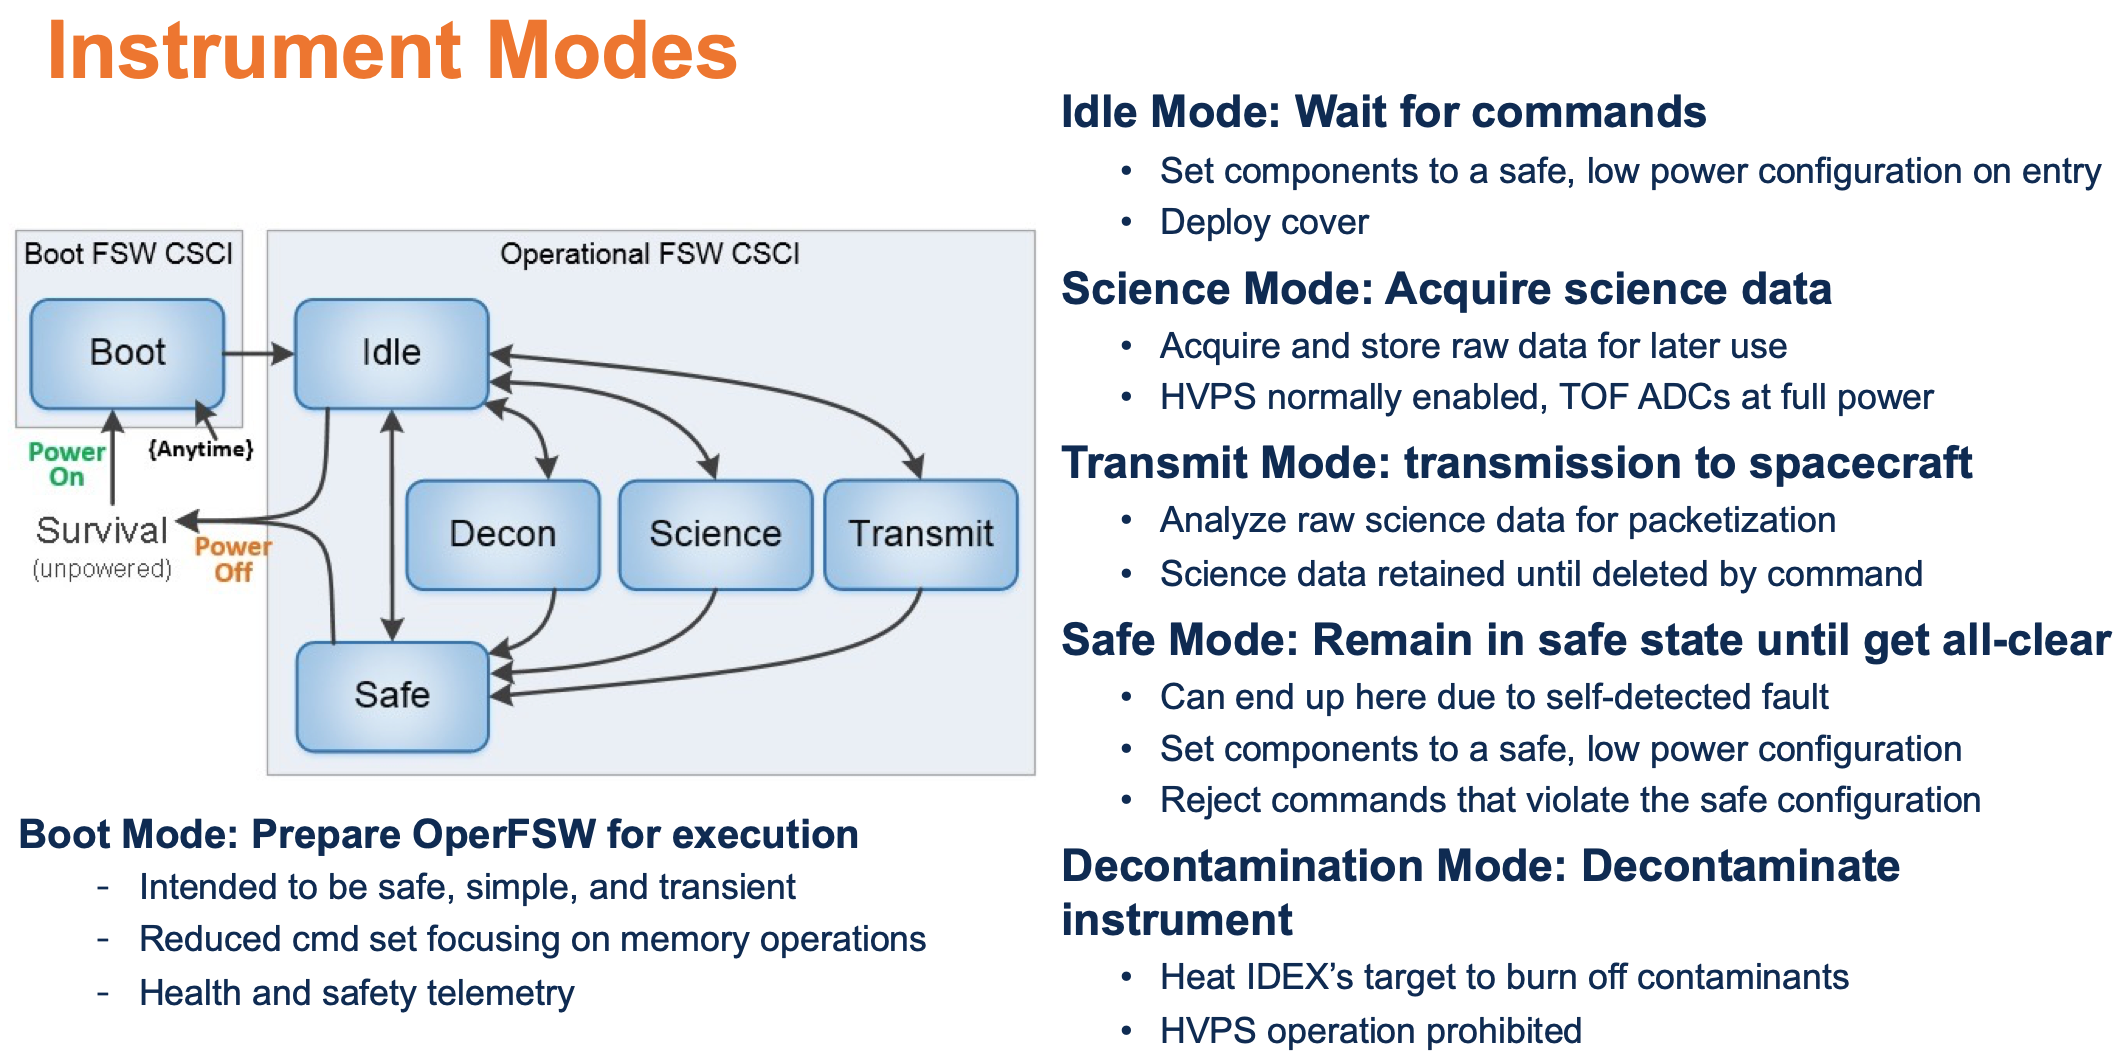
\includegraphics[width=\linewidth]{images/operation.png}
    \caption{An outline of the IDEX instrument operation modes.}
    \label{fig:oper}
\end{figure}


The \textbf{boot} mode is enabled when the instrument is powered on or any other time the operator indicates. In this mode, while FSW is performing a set of memory operations to prepare for execution, a health and safety telemetry packet is transmitted.

Following boot, the instrument enters its \textbf{idle} mode, %where the door is deployed 
and the instrument awaits commands. From here, the instrument may enter one of four possible operational modes, of which only two are relevant to the science data processing pipeline.

\subsection{Science Mode}
When the instrument enters the \textbf{science} mode, a memory buffer is continuously filled containing each of the 6 instrument signals. Since IDEX is an event-driven instrument, data is only packetized and transmitted when we have a dust impact, which we will refer to as an \textbf{event}. The instrument triggers based off of an event, sending the data stored in the memory buffer to the NAND flash.

The amount of data stored in a memory buffer depends on the sampling rate of the corresponding \textbf{analog-digital converter (ADC)}. The three time-of-flight gain stages are sampled at 260 MHz (high sampling rate). The two target gain stages and the ion grid, the ADCs are sampled at 4 MHz. Figure \ref{fig:pack} illustrates how data is packed for these two types of ADCs, as well as how much data is transmitted per event.

\begin{figure}[H]
    \centering
    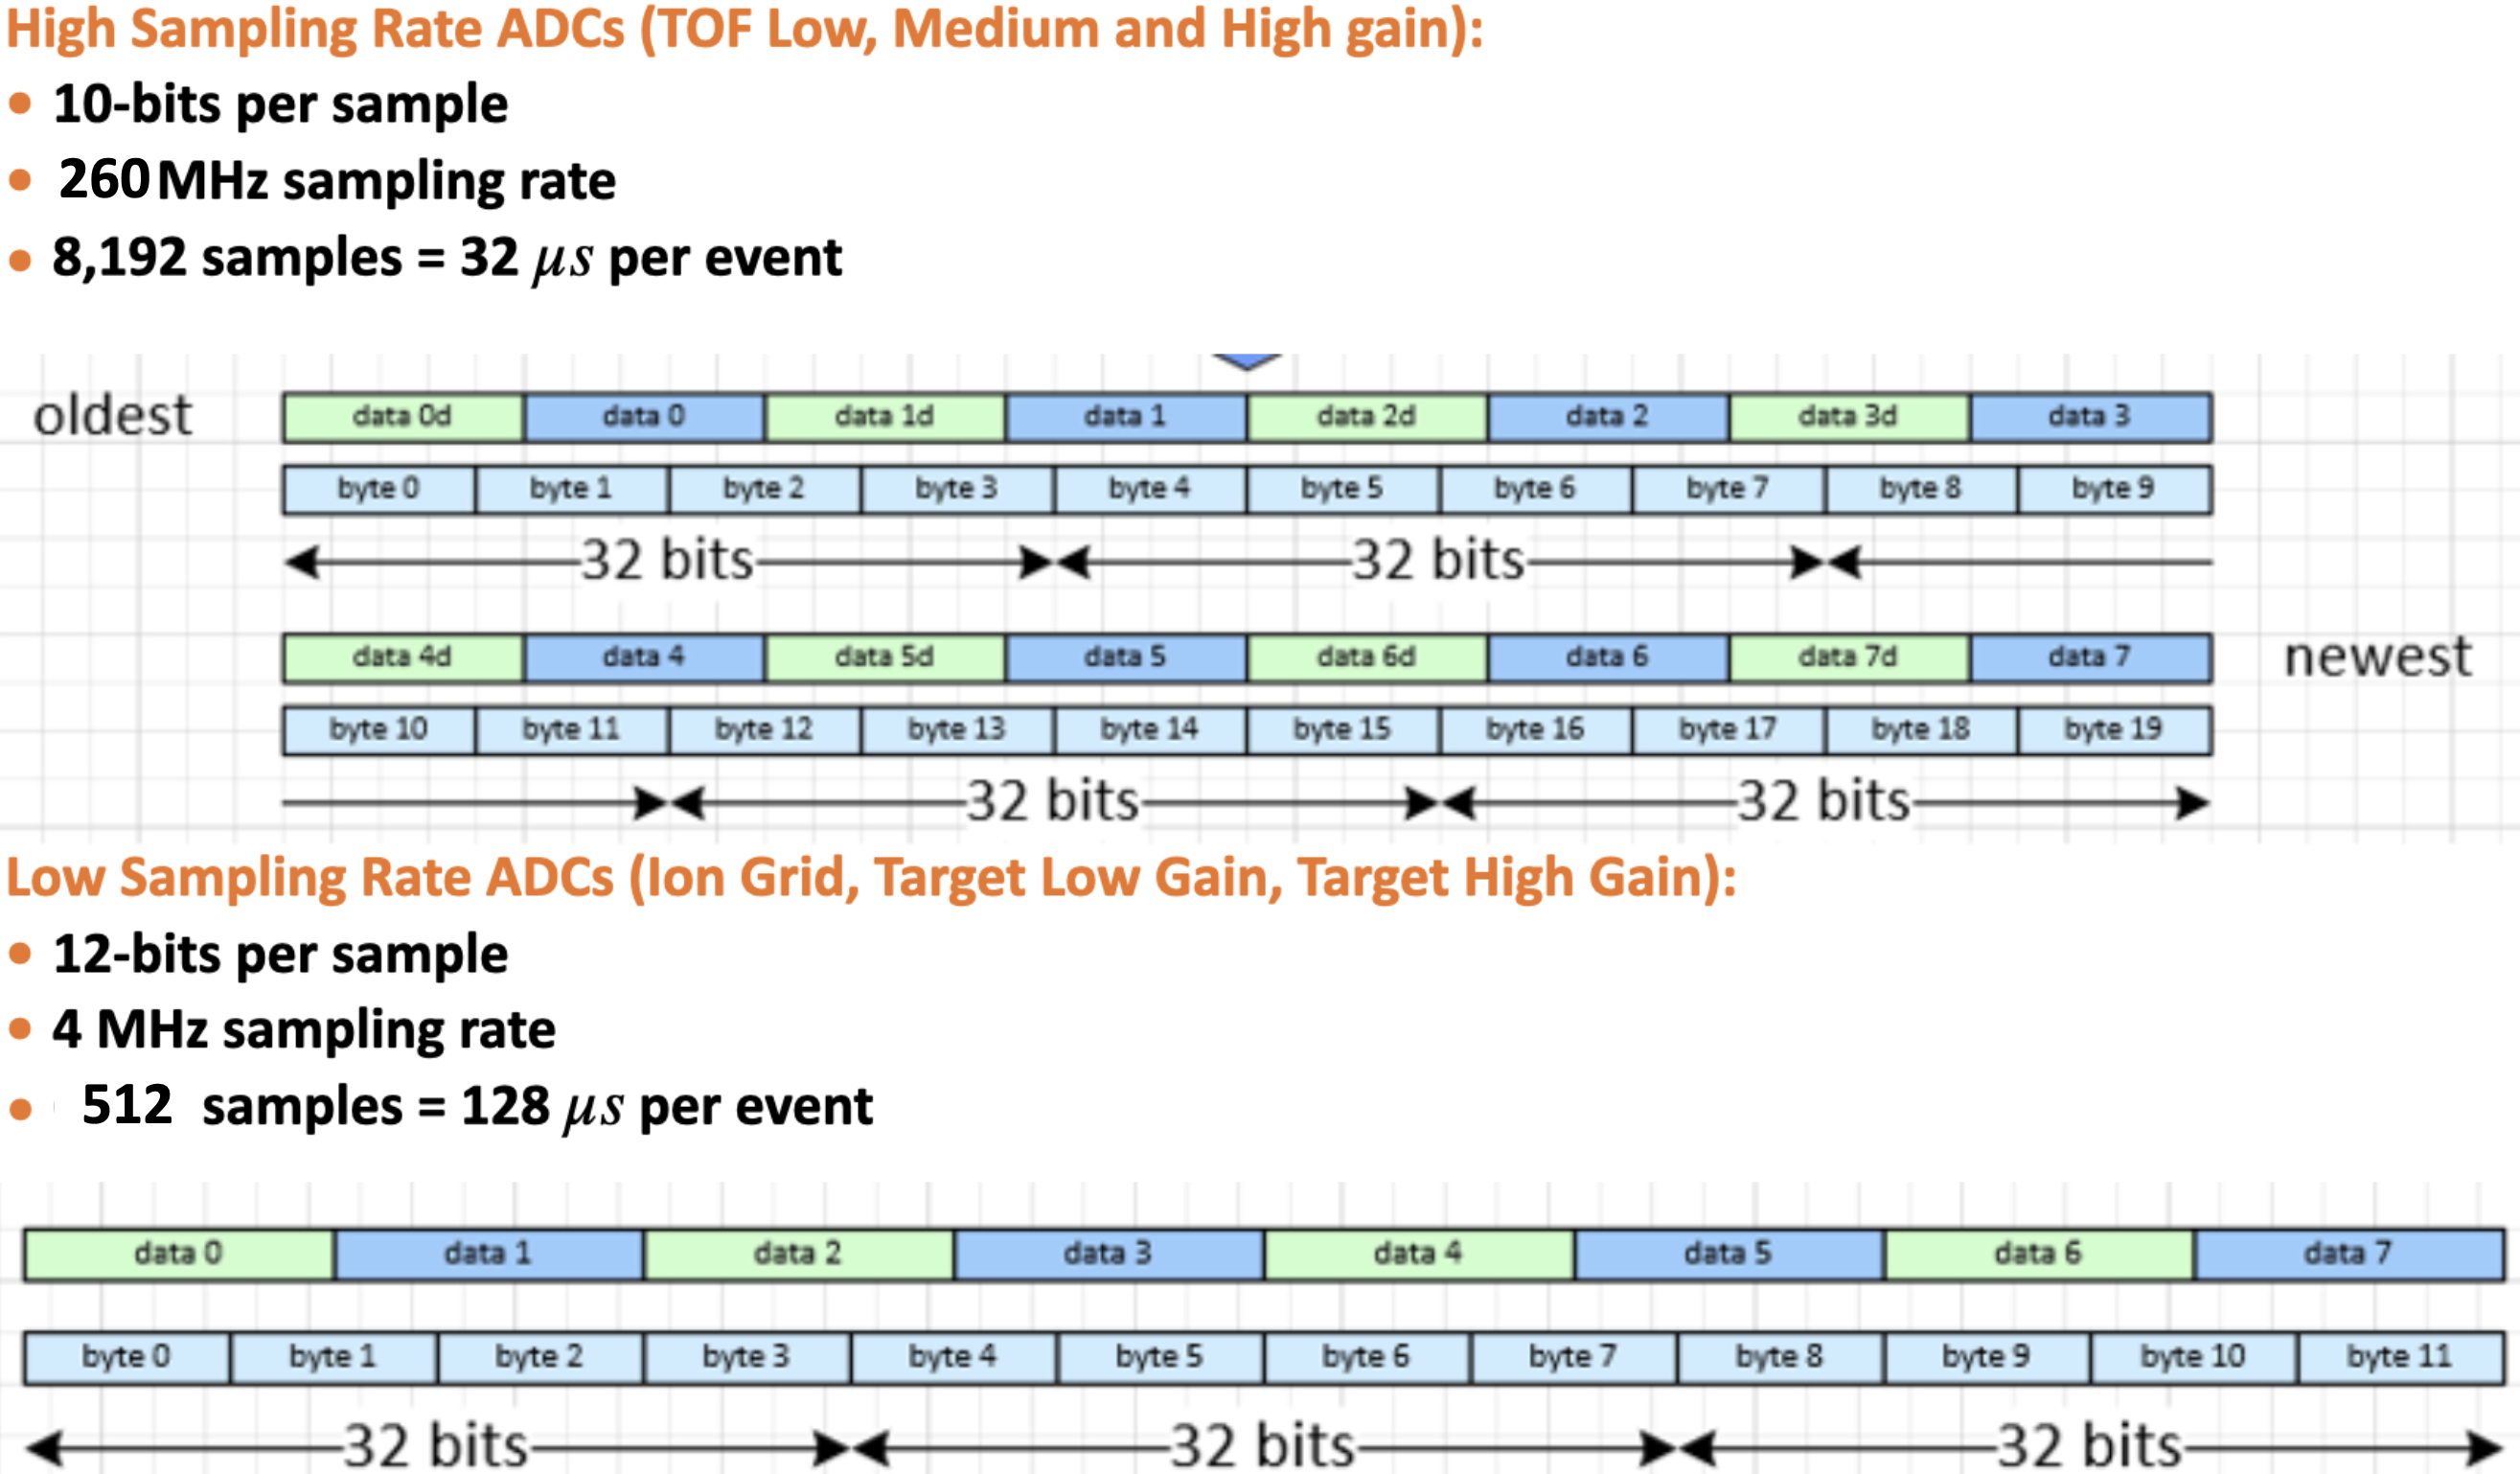
\includegraphics[width=\linewidth]{images/datapackaging.png}
    \caption{Diagram illustrating how data from the two different ADCs is packed in the NAND flash. Each event generates 88,064 bits of waveform data.}
    \label{fig:pack}
\end{figure}

\subsection{Transmit Mode}
Once the NAND flash has been populated with data from all 6 signals, it is ready for transmission. There are additional  post-trigger blocks based on the sampling rate of the corresponding ADCs, as pictured in Figure \ref{fig:adcf}.

\begin{figure}[H]
    \centering
    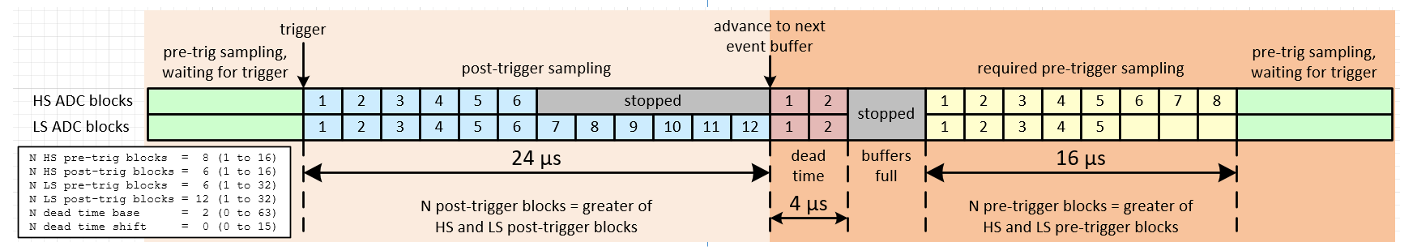
\includegraphics[width=\linewidth]{images/adcflow.png}
    \caption{Block diagram of the instrument timeline, based on high (HS) and low (LS) sampling rate ADCs.}
    \label{fig:adcf}
\end{figure}

Once the instrument triggers, there is a 4 $\mu$s dead time after the required post-trigger sampling has been completed. Hence,  at the very least, there will be a 4 $\mu$s gap between events. 

%This dead time is also optional if the instrument is expected to receive a high particle count.  NOT SURE WHAT THIS MEANS? CAN IDEX TURN OFF DEADTIME?

Transitions between instrument modes are driven by commands from the spacecraft. For the purposes of error detection and correction (EDAC), the 30 most recently executed commands and their associated timestamps are stored in the instrument log. This instrument log can be telemetered to the ground with the \textbf{DumpLog} command. These 30 commands include successful and failing command executions. However, if the command is so badly mangled that the FPGA or FSW is unable to recognize it as a command, then it does not get included in the log. %IS THERE A COUNTER FOR THESE ?

\subsection{Spacecraft Time Interface}

Each event is organized chronologically by the FPGA trigger time. For each event, the trigger time is stored in the event header. The event header is always specified by \textbf{SCI0TYPE=1} (see \ref{sci} for more details). This is given by a linear combination of the \textbf{SHFINE} and \textbf{SHCOARSE} variables. For each FPGA header, the \textbf{SHCOARSE} variable is a 16-bit unsigned integer that delineates the number of seconds since epoch (Midnight, January 1st, 2012)\textbf{SHFINE} variable indicates a number of 20 microsecond intervals in addition to the seconds since epoch.
Together, these time measurements establish when an event took place with respect to epoch. The formula to retrieve the epoch from the FPGA header is given by 

\begin{equation}
    \tau_{epoch} = SHFINE + 20*10^{-6}*SHCOARSE
\end{equation}

Additionally, the time axis for each of IDEX's 6 signals is derived from the sampling rate and the number of samples. The Ion Grid and two Target waveforms sample at 4 MHz, and the TOF sample at 130 MHz. The number of samples can then be multiplied by $3.846 \,[n s]$ and $246.15 \,[n s]$ for the time axis. \textbf{These samples are packed into blocks of 512 samples for the high sampling (HS) rate data and 8 for the low sampling (LS) rate data. The maximum amount of high-rate data is 16 blocks, which would be 8192 samples covering 31.5 us of time. The maximum amount of low-rate data is 64 blocks, which would be 512 samples covering 126.03 us of time.}
 
To line up the data, you need to line up the trigger point based on the settings for pre-trigger blocks and post-trigger blocks for the high-rate and low-rate data. For this, we turn to the \textbf{NBlocks/TXHDRBLOCKS} variable in each FPGA header. This variable is interpreted according to the map in figure~\ref{fig:nblocks}.

\begin{figure}[H]
    \centering
    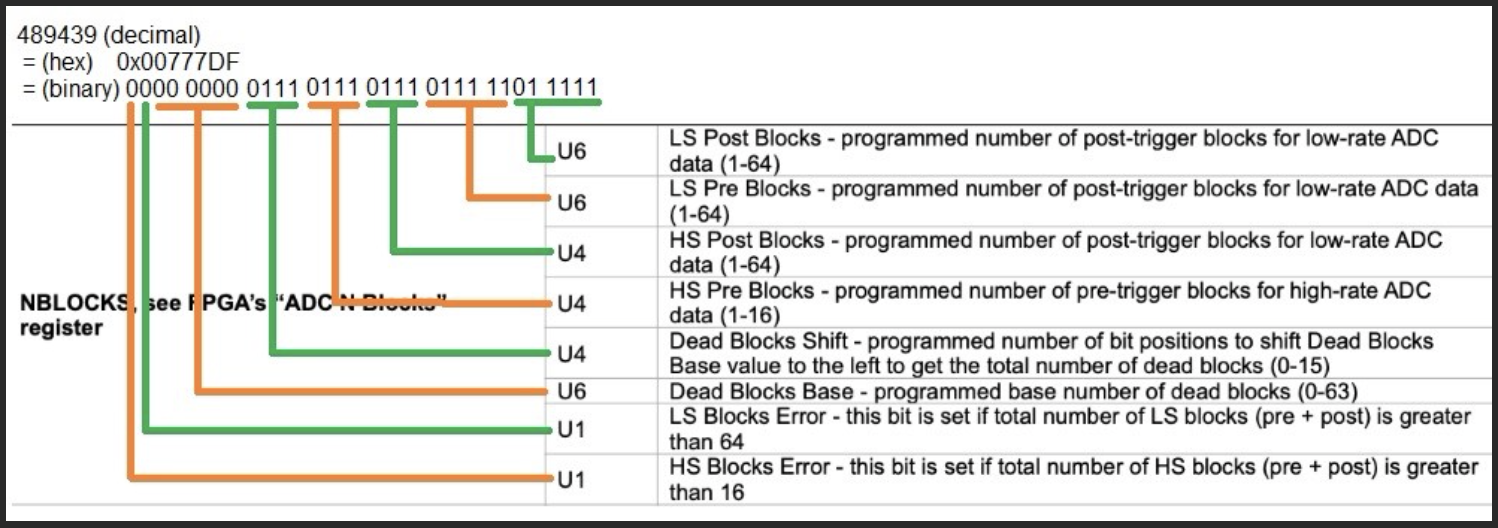
\includegraphics[width=\linewidth]{images/nblocks.png}
    \caption{Map showing how to decompose the \textbf{NBlocks} variable, provided by Greg Newcomb.}
    \label{fig:nblocks}
\end{figure}

The example shown is for a given integer value used during early integration and test, where the trigger was always in the middle of data acquisition (same number of pre and post trigger samples). Generally, this variable is a 32 digit binary string, which can be broken down as follows:

\begin{mdframed}[backgroundcolor=backcolour]{
 {\bf Digit 1} = 1 or 0 if there is an issue with the number of HS blocks. \\
 {\bf Digit 2} = 1 or 0 if there is an issue with the number of LS blocks. \\
 {\bf Digits 3-8} = Programmed base number of dead blocks: after post trigger sampling? \\
 {\bf Digits 9-12} = Dead blocks shift: Used with 3-8 to determine total number of dead blocks. \\
 {\bf Digits 13-16} = Number of high sampling pre-trigger blocks. \\
 {\bf Digits 17-20} = Number of high sampling post-trigger blocks. \\
 {\bf Digits 21-26} = Number of low sampling pre-trigger blocks. \\
 {\bf Digits 27-32} = Number of low sampling post-trigger blocks. \\
} \end{mdframed}

\section{Nominal Science Operations}
IDEX is an event-driven instrument, so data collection only takes place in the event of a trigger. Otherwise, when in science mode the instrument will continuously fill and delete the memory buffer. 



\section{Data Products}
The IDEX science data products pipeline takes raw instrument CCSDS packets (level 0 data) as inputs and goes through each stage of the mass spectrum calibration process to reveal the composition, target impact charge, and ion-grid charge of each measured dust particle (level 3 products). Each science data product level is delineated below in 
Table~\ref{fig:levels}.
\begin{table}[H]
    \centering
    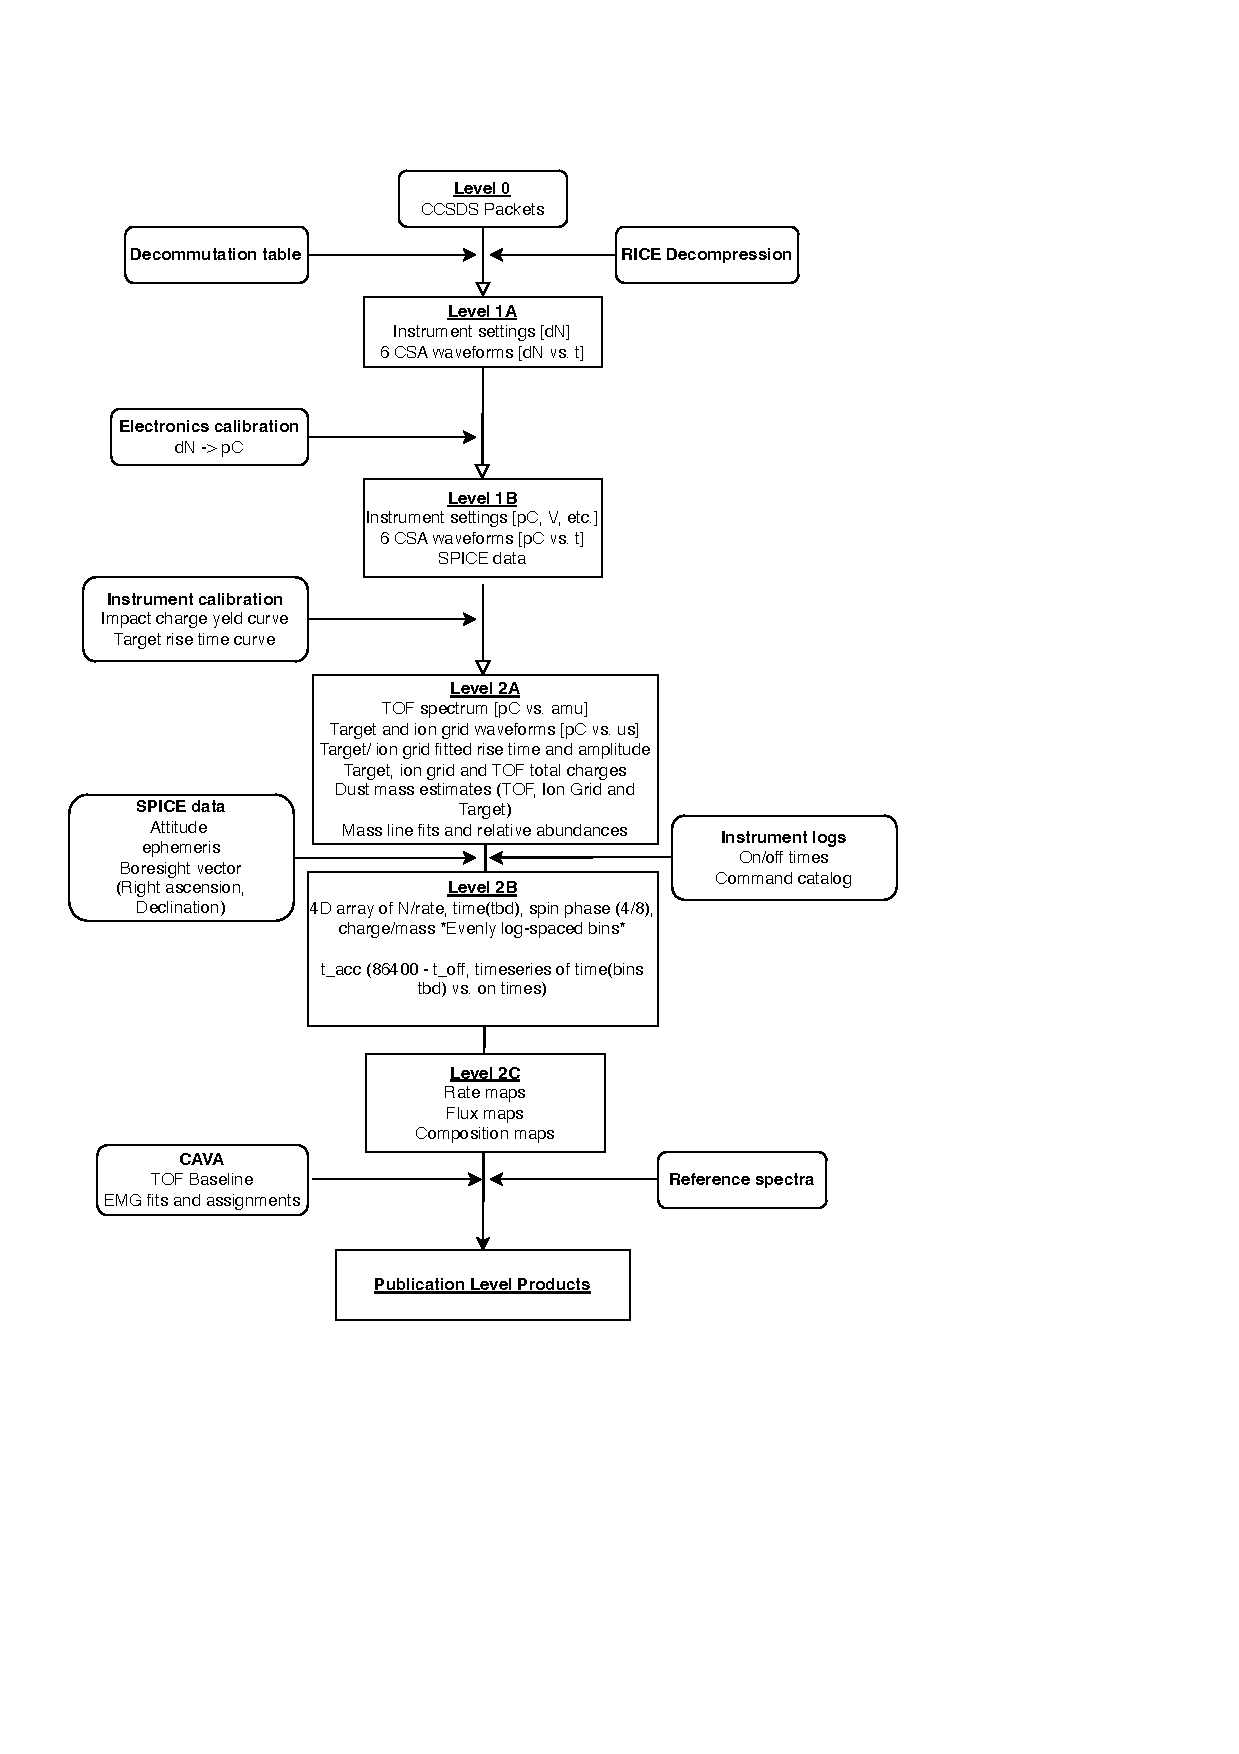
\includegraphics[width=.7\linewidth]{images/PipelineFlow_Updated.key.drawio.pdf}
    \caption{An outline of the IDEX instrument science data product levels, their format, and a brief description.}
    \label{fig:levels}
\end{table}

\subsection{Science Data}
\label{sci}
IDEX generates three APIDs containing science data:
\begin{itemize}
    \item \textbf{Transmit (APID 0x590):} Waveforms and metadata for science events, in response to the \textbf{Transmit} command.
    \item \textbf{Fetch (APID 0x591):} Waveforms and metadata for science events, in response to the \textbf{Fetch} and \textbf{FetchOne} commands.
%    \item \textbf{Catalog (APID 0x592):} Catalog summarizing characteristics of science events for one dataset, in response to the \textbf{SendCatalog} command. (Not implemented for IDEX) %but is available). ????? DO WE DEFINE CATALOG ENTRIES - WHAT IS AVAILABLE?

    
\end{itemize}
The contents of each APID are further described below.  All IDEX packets are 32-bit aligned, starting with a CCSDS header. only APID 0x590 is expected to be used by IDEX.  All IDEX packets are 32-bit aligned, start with a CCSDS header, and end with a 2-byte CRC.  Each IDEX packet is encapsulated in an interface transfer frame (ITF) required by the IMAP General Instrument to Spacecraft Interface Control Document (GI ICD, APL \#7516-9055), but is ignored in this document.
\vspace{.1 in}

In general, science data is organized onboard by the \textbf{accountability identifier (AID)}.  The AID is assigned when the data is acquired, and is used to access the data afterwards.  The AID cannot be changed, and duplicate AIDs are not permitted.  Each dataset is composed of one or more \textbf{“events”}, which is a collection of data collected when the instrument triggers, usually representing a dust particle impact.  Each event is given a unique “event number” by the FPGA, so that every event collected by IDEX can be uniquely identified by the combination of AID and event number. 
\newline





Event data is composed of seven distinct parts:
\begin{enumerate}
\item	Time of Flight (TOF) waveform data on the high-gain (HG) channel, sampled at 260 megasamples per second (Msps) with 10-bit resolution.
\item	TOF waveform data on the mid-gain (MG) channel, sampled at 260 Msps with 10 bit resolution.
\item	TOF waveform data on the low-gain (LG) channel, sampled at 260 Msps with 10 bit resolution.
\item	Ion (ION) grid Charge Sensitive Amplifier (CSA) waveform data, sampled at 4.0625 Msps with 12 bit resolution.
\item	Target Low Range (TLR, AKA target high gain) charge sensitive amplifier (CSA) waveform data, sampled at 4.0625 Msps with 12 bit resolution
\item	Target High Range (THR, AKA target low gain) charge sensitive amplifier (CSA) waveform data, sampled at 4.0625 Msps with 12 bit resolution
\item	FPGA Pre-pended metadata header containing IDEX’s configuration and status at the time of the trigger, recorded by the FPGA.
\end{enumerate}
\begin{figure}[H]
    \centering
    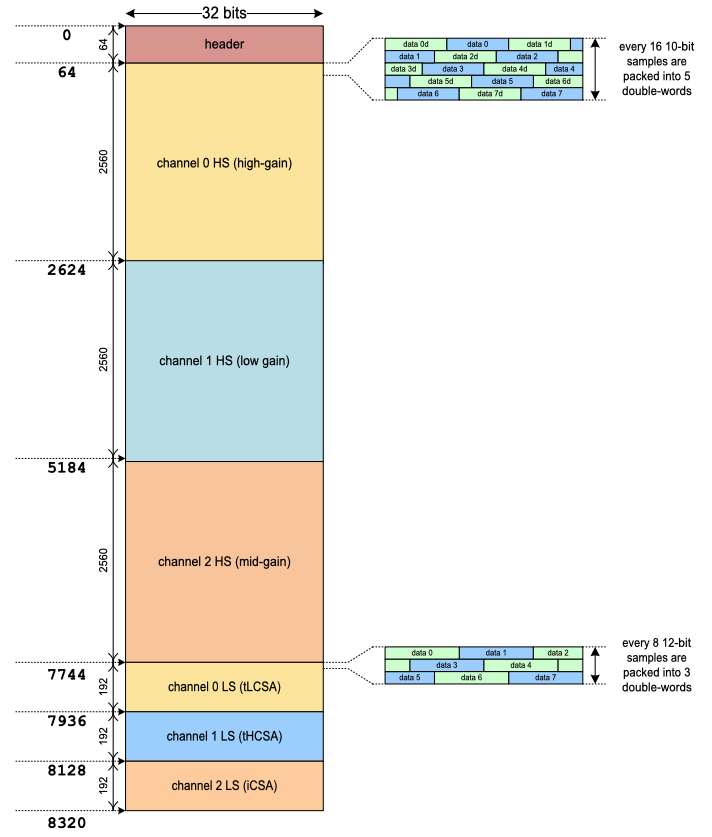
\includegraphics[width=.8\linewidth]{images/waveformdata.png}
    \caption{A bitmap outline of the science data constituting each event}.
    \label{fig:head}
\end{figure}

At the end of science data acquisition, a catalog %WHAT IS IN THE CATALOG?  DO WE DEFINE SPECTRA TYPES ???
representing the new dataset is stored along with the raw science data in nonvolatile memory.  The catalog is mostly empty at this point but can be downlinked with the \textbf{SendCatalog} command.  If no science data is acquired during acquisition, then no catalog is created either. A high-level diagram of how the high and low sampling rate ADC data is transmitted once packetized is shown in Figure \ref{fig:head}, describing how different blocks of data are stored.


Following science data acquisition, FSW will transmit the science data with the “Process\_Transmit” command using APID 0x590. . Processing is started with the \textbf{Process} command, which has the FSW evaluating waveform data to determine characteristics (e.g. peak count) of each event. The characteristics are then used to assign each individual event to a category. As each event in a dataset is processed, a new entry is added to the catalog (in chronological order of acquisition). The FSW includes a setting where event data (all seven parts) are transmitted (APID 0x590) as soon as it is processed – which was used for some early ground testing but never afterward.\newline
A dataset only needs to be processed once but can be processed multiple times (with different results if parameter table entries%DEFINING INSTRUMENT SETTINGS? CHANGED BY WHO WHEN?)
are changed).  However only the most recent processing results are saved to the catalog.\newline
Once a dataset is processed, it can be downlinked as any of the three packet types. Normally the catalog is sent right away since it is considered “feed-forward data” used to configure instrument parameters for subsequent data acquisition opportunities. “Transmitted” science data comes next, and are used as a “first pass” at evaluating the science data and downlinking a subset of acquired events. Afterward, scientists will evaluate the catalog and request specific events to be downlinked as “fetched” science data. Another option is that the dataset can be “transmitted” again but with different parameter table entries resulting in a different selection of events transmitted. %IDEX IS NOT DOING THIS >>>>>PERHAPS ALL CATALOG RELATED STUFF SHOULD BE LEFT OUT?
\newline

\subsubsection{Transmitted and Fetched Science Packets}
Transmitted and fetched science data share the same decommutation, the only real difference being the APID.  When transmitting or fetching science data, one event is handled at a time. Each event may spawn between 1 and 10 packets, depending on size and requested contents. %THIS TOO ONLY MAKES SENSE IF WE HAVE A CATALOG?
\newline
As mentioned above, event data is composed of seven distinct parts but not all are sent for every event.  An argument of the \textbf{FetchOne} command specifies which parts to send, and similarly the Fetch Table includes this info for “Fetch” commands (see \textbf{AddToFetch} command for more details).  Parameter table entries are used to determine what parts of an event are sent for transmitted data (using the event’s category which themselves are grouped into quality factors). % IS THIS  RELEVANT TO IDEX?  MAYBE THERE SHOULD BE A SEPARATE SECTION FOR THE CATALOG STUFF, WHAT IS CATALOGED AND HOW THIS COUD BE USED, AND THAT IT IS NOT EXPECTED TO BE EXERCISED\newline
Each part of the event is packaged into its own packet, while still sharing the same APID.  To fit within the IICD-required maximum CCSDS packet length of 4095 bytes, one packet will contain no more than 4032 bytes of science data (the rest dedicated to headers and such). Each part normally fits in one packet, but the TOF waveforms can span two-three packets if the dataset is large and compression is poor (or disabled). In this case, the maximum amount of science data is sent in the first packet and any leftover sent in the next packet.
The content of packets containing the metadata header are very different from the waveform data, so it is discussed separately.\newline

\subsubsection{Packets Containing Waveforms}
Science packets containing any of the six waveforms, whether transmitted or fetched, start with a brief header and are followed by a variable amount of science data.  The header is never compressed, and provides identifying information such as AID, event number, and which waveform.  \newline
\label{wavepack}
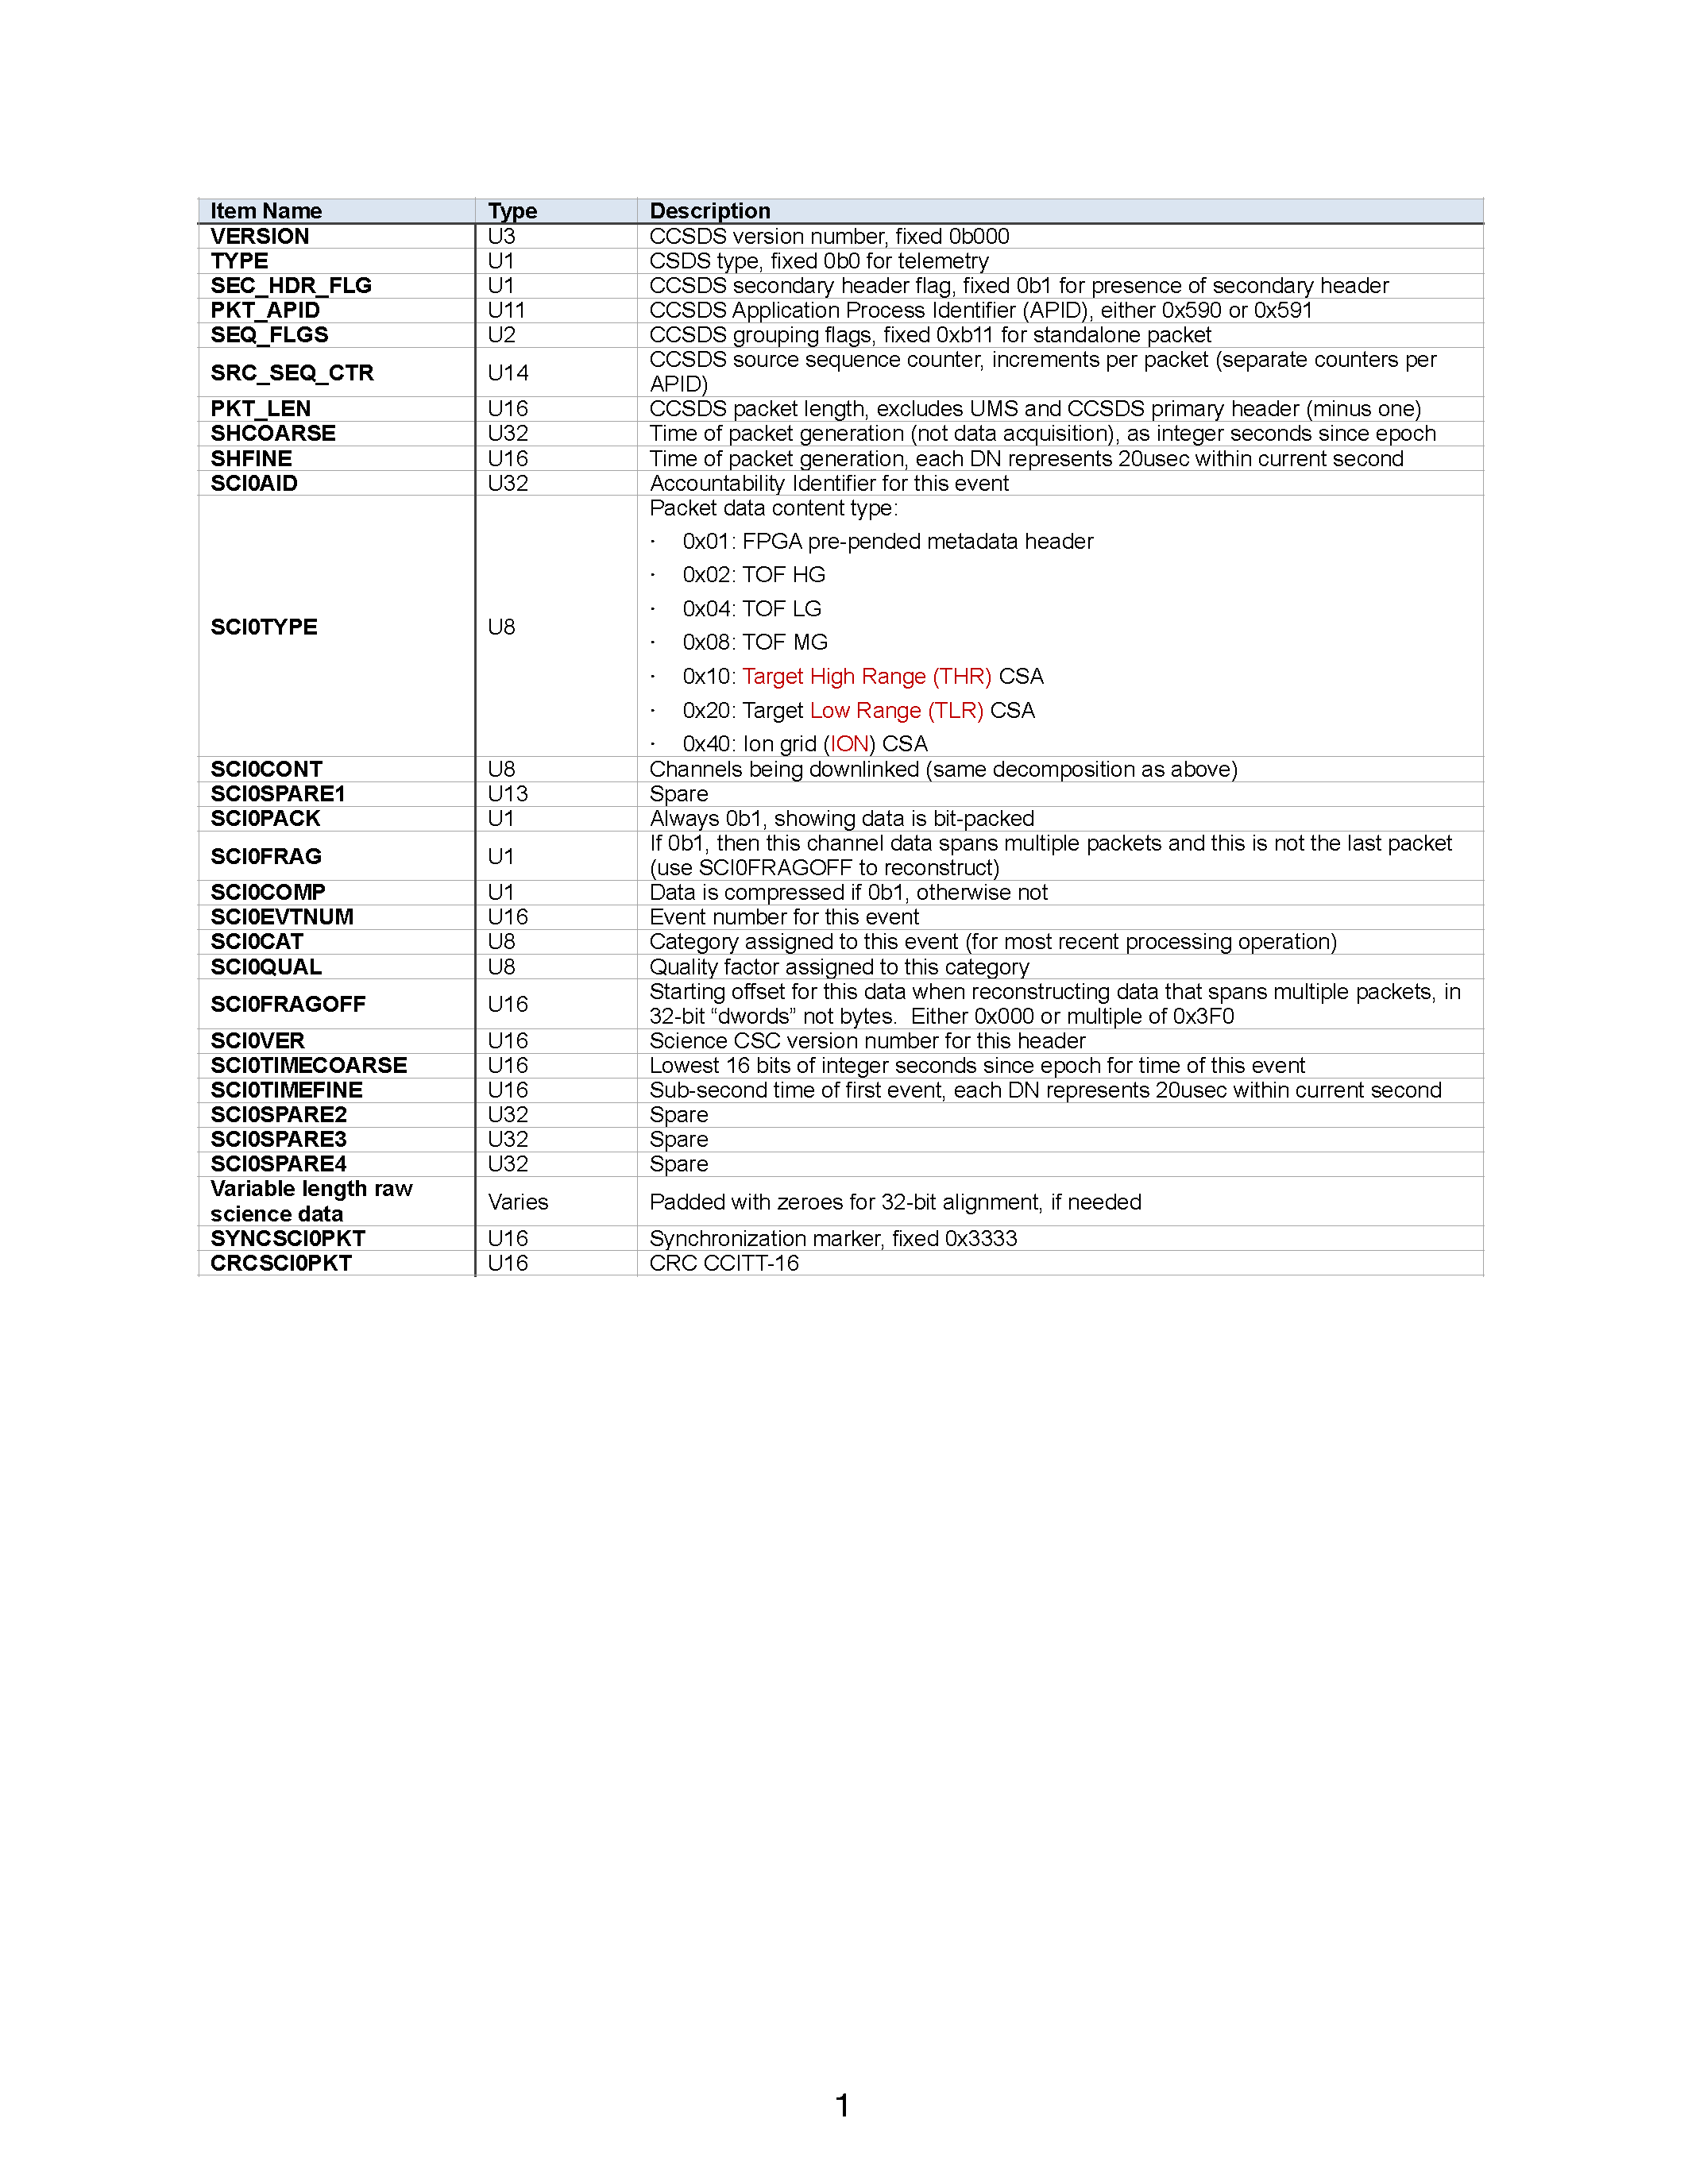
\includepdf[pages=-,pages=1, 
  pagecommand={},
  trim=0 2cm 0 0,
  clip,width=1.25\textwidth]{images/waveformpackets.pdf}

Outline of fields in waveform-containing packets. Red text indicates changes from the SUDA definitions.


\begin{figure}[H]
    \centering
    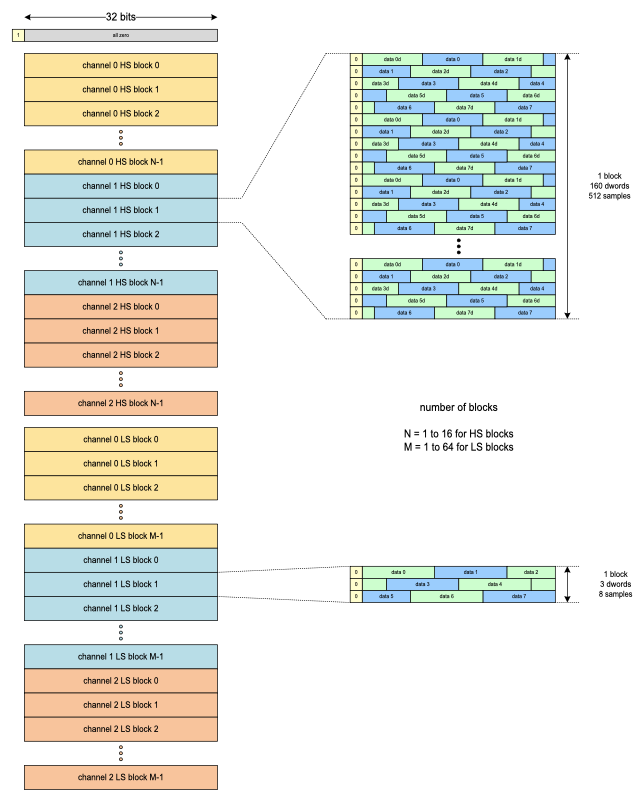
\includegraphics[width=.8\textwidth]{images/wavebreak.png}
    \caption{A bitmap outline of what is contained in each set of waveform data.}
    \label{fig:wavebreak}
\end{figure}

The FSW can make use of the FPGA’s RICE compression core, with details discussed in the FPGA specification (167130). \textbf{If the resulting compressed data is not 32-bit aligned, then the remainder (up to 31 bits) are padded with zeroes}. To decompress a TOF waveform, a RICE decompressor should be used and the output interpreted as a chronological series of 10-bit samples. For SCA %???%
waveforms, the output is 12-bit samples.\newline
After the data is decompressed on the ground, the resulting data represents 6 time-ordered waveforms corresponding to each AID.


The packet is summarized in the table below, using a format similar to the SUDA Command and Telemetry handbook:
\begin{itemize}
    \item Item name: Mnemonic for the named item
    \item Bytes: Position of the item within the element, show bytes with packet and bits within byte
    \item Type of data: Everything is “U” for unsigned data number, followed by bit length
    \item Description: Briefly describes the item, giving the conversion if appropriate.
\end{itemize}
The \textbf{SCI0RAW} field contains the instrument waveforms in each packet. How the header, low sampling and high sampling rate ADC data appears in each packet is described in figure \ref{fig:wavebreak}.
While each channel appears in 3 packets for most events, figure \ref{fig:wavebreak} describes the general case for $N$ high sampling and $M$ low sampling blocks. Each packet header, on the other hand, is only contained in one packet.

\subsubsection{Packets Containing FPGA Metadata Headers}
The packet containing the metadata header holds status and configuration information at the time when this event was acquired. This includes the voltages, currents, temperatures and other instrument settings at trigger time. eThe first 32 bytes after the CCSDS header are identical to the preceding waveform data, so that the SCI0TYPE field can be used as a key to differentiate packets containing this metadata header versus waveforms.

After the common header is the \textbf{FPGA prepended metadata header} that the FPGA captures for every event. These data are fixed size and never compressed.  Many of these fields are the same for all events within the same dataset. A diagram describing the components of the FPGA header is shown in Figure~\ref{fig:headbit}.

\begin{figure}[H]
    \centering
    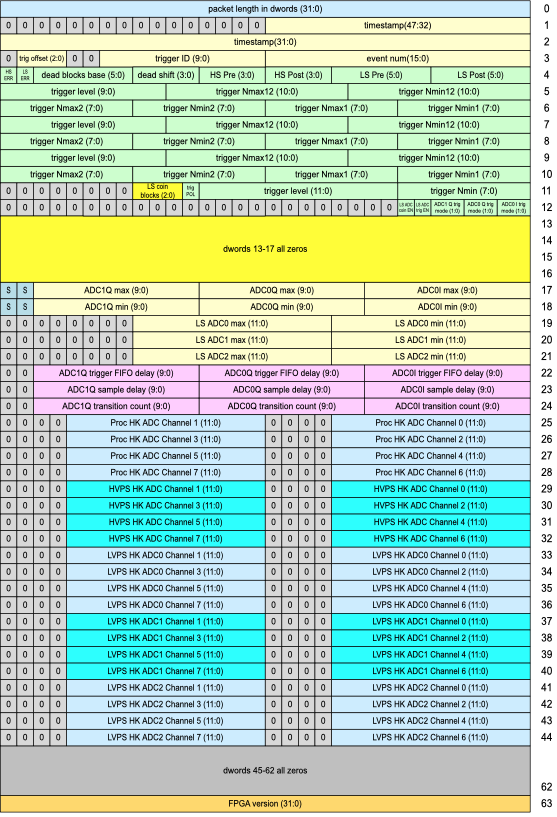
\includegraphics[width=.7\textwidth]{images/HeaderBitmap.png}
    \caption{A bitmap outline of what is contained in each FPGA  metadata event header.}
    \label{fig:headbit}
\end{figure}
The fields in the FPGA header pertinent to the level 0 to 1 science data processing pipeline include the \textbf{timestamp}, \textbf{event num}, and various \textbf{trigger} fields. A full outline of all the available fields including their length, dtype, and description is shown below.

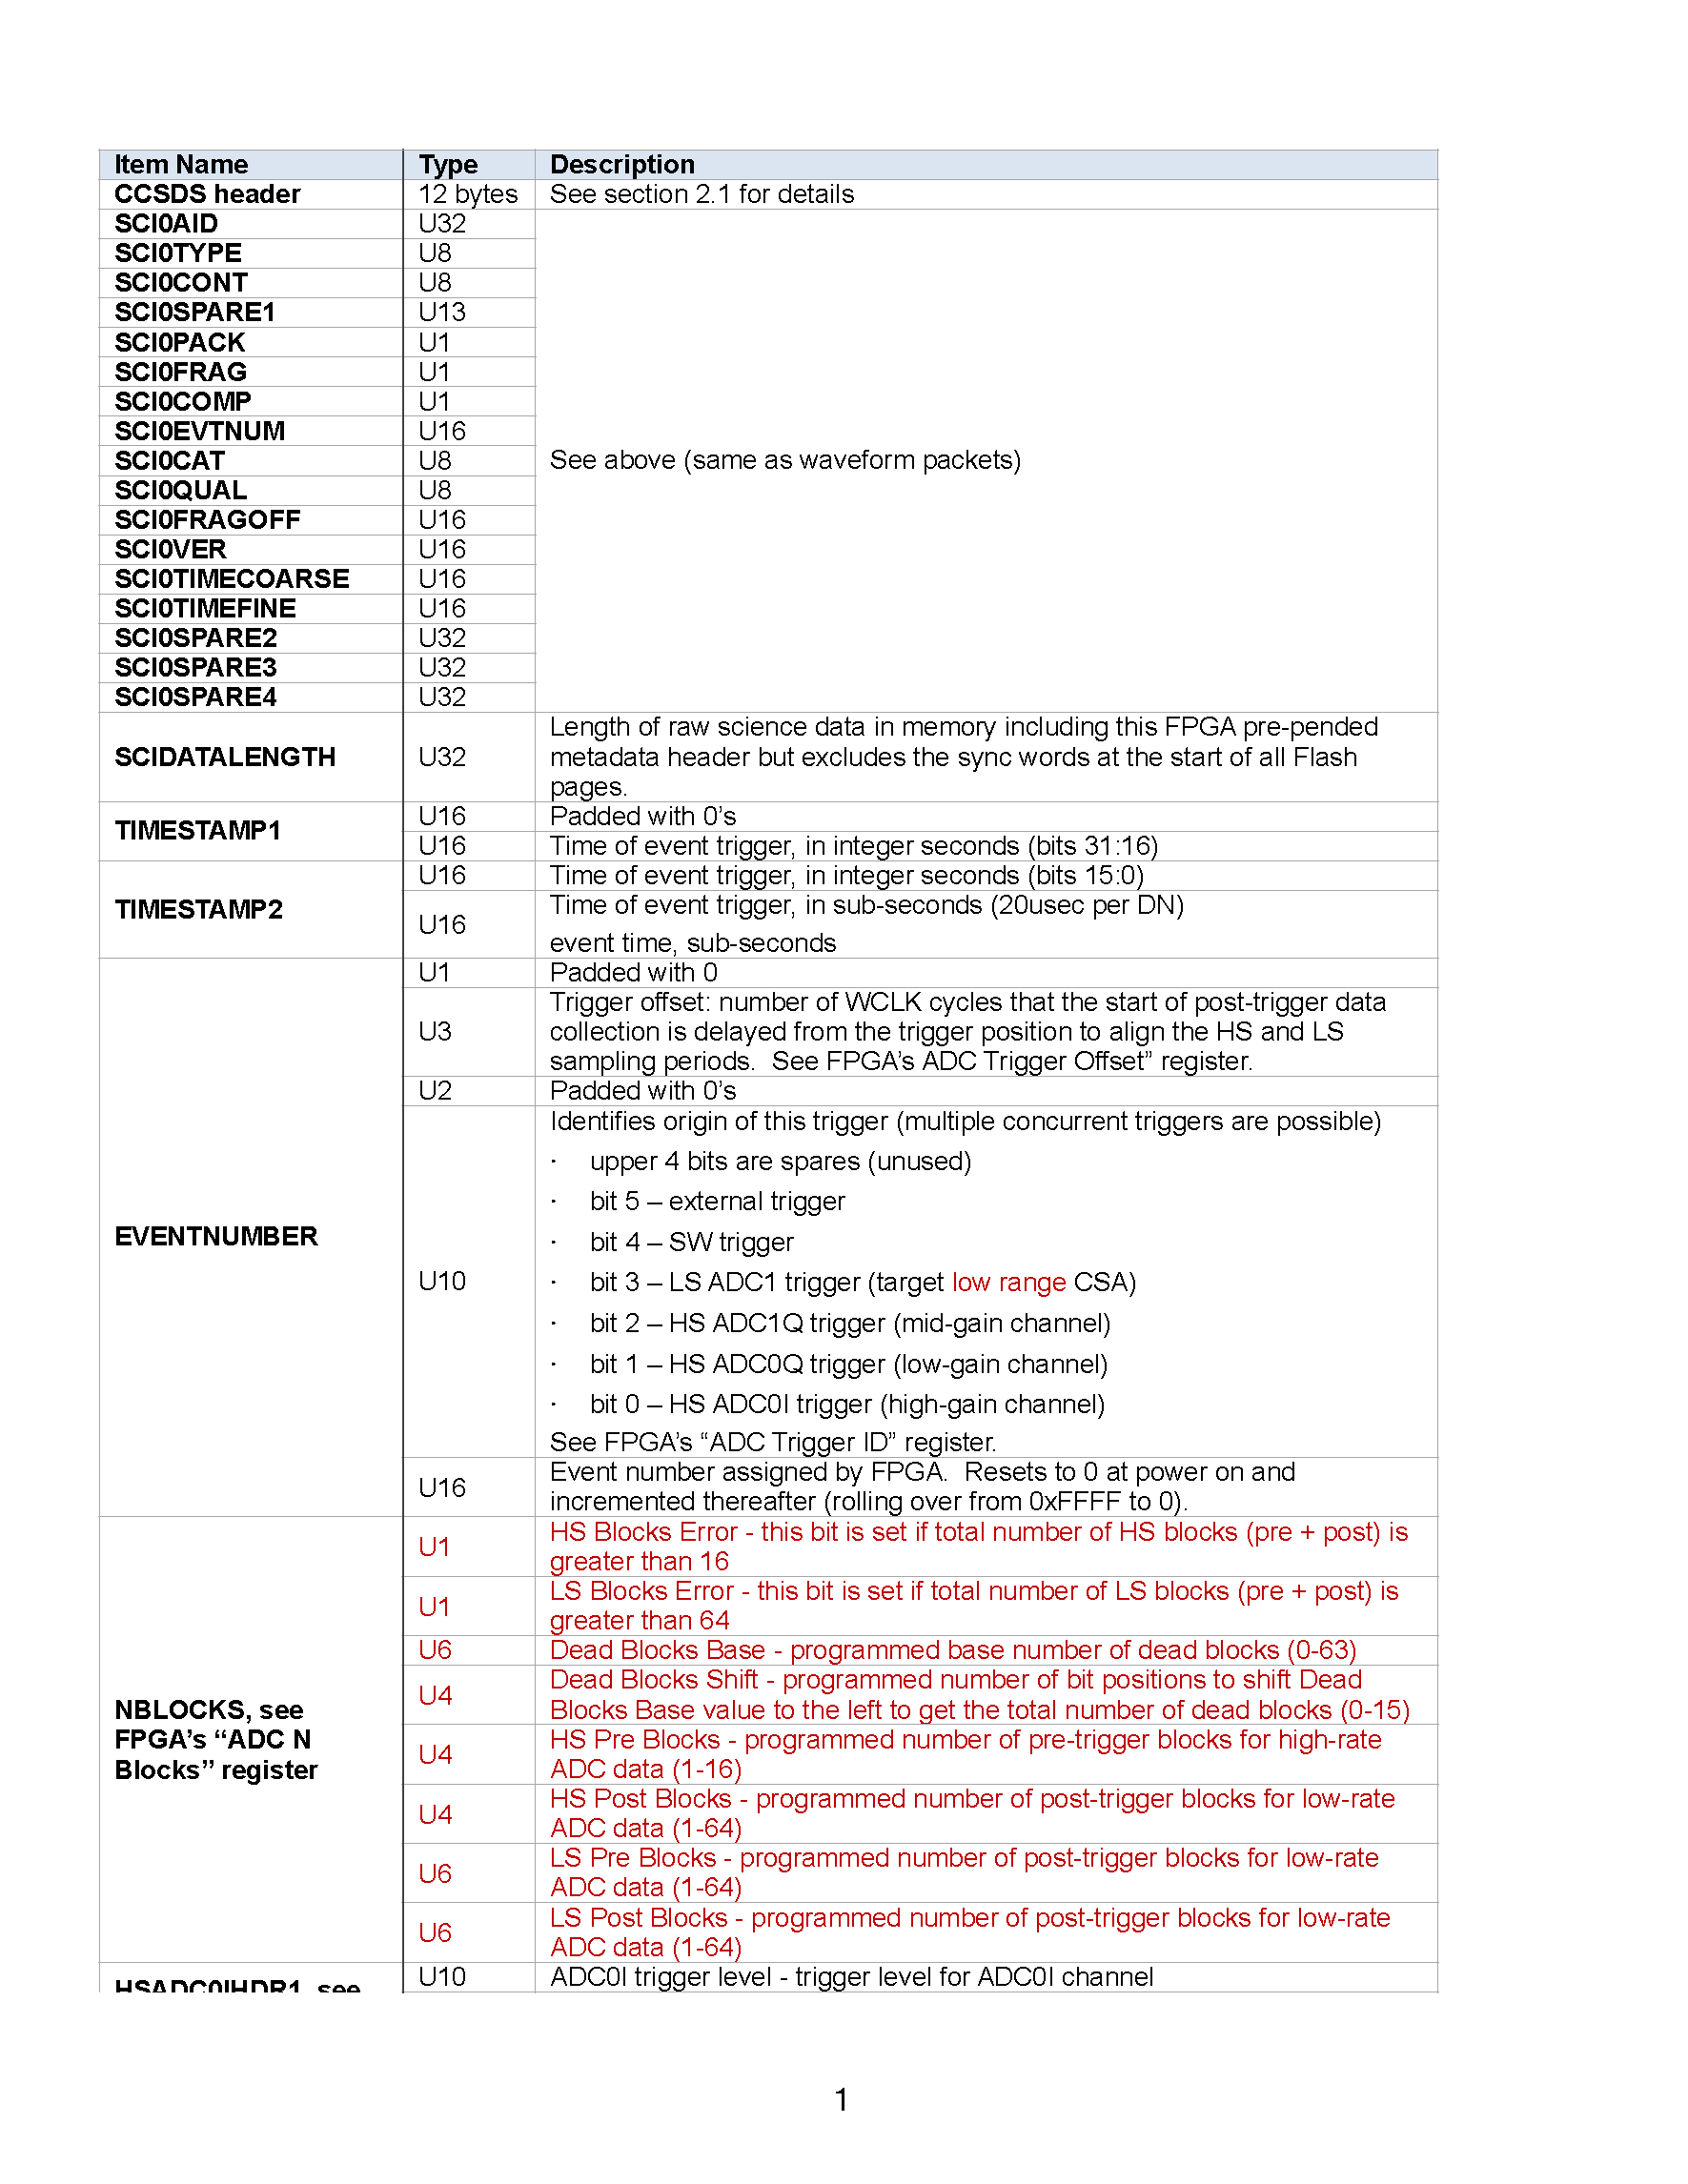
\includepdf[pages=-,width=1.25\textwidth]{images/headerpackets.pdf}


% \subsection{Housekeeping Data}
% ***UPDATE IN FUTURE DRAFT***
% \subsection{Engineering Mode Data}
% ***UPDATE IN FUTURE DRAFT***
% \subsection{In-Flight Calibration Data}
% ***UPDATE IN FUTURE DRAFT***

